% !TeX program = lualatex

\documentclass[12pt]{report}

\usepackage{url}
\usepackage{hyperref}

\usepackage{graphicx} % images
\usepackage{subcaption}

\usepackage{fontspec}
\setmainfont{Times New Roman}

\linespread{1.25} % the equivalent of 1.5 line spacing from msword

% margins
\usepackage[a4paper, left=2.5cm,right=2.5cm,top=2.5cm,bottom=2.5cm]{geometry} 

\usepackage{amsmath}

\usepackage[]{algorithm2e}

\usepackage{todonotes}

\begin{document}
	\listoftodos
	
	\title{Skin detection in images using machine learning techniques for color and texture recognition}
	\author{Stefan Sebastian}
	\date{\today}
	\maketitle
	
	\newpage
	\tableofcontents
	\newpage
	
	\chapter{Introduction TODO}
	
	\section{Introduction}
	Skin detection means identifying pixels and regions in images which correspond to human skin. Starting from these regions we can build models that detect people or certain body parts.
	
	There are many challenges in creating a good skin detector. One of the most challenging aspects is handling illumination. While the human eye can easily distinguish the same color in varying degrees of brightness this is not a trivial task for computers. The second aspect we must consider are the variety of skin tones. A good model should be able to handle people of all races. Another thing to note is the fact that there are a lot of objects and materials that resemble skin such as leather, wood, sand etc. Consequently, most models have a rather large false positive rate (around 10\%).
	
	The purpose of this paper is to present the best models currently employed in skin detection and to propose a new model that combines some state of the art detectors. To the best of my knowledge no method that combines image segmentation, color and texture analysis has been published in this area of research. For every approach in skin detection I included a theoretical introduction followed by some examples of its practical use in skin detection.
	
	\section{Applications}
	One of the first applications in this field of study was scanning internet images in order to filter pornographic content \cite{finding_naked_people}. The model proposed in that paper scans the images for large areas of skin and then applies some geometrical analysis looking for elongated shapes.
	
	Another application was detecting anchorpersons in talk shows \cite{anchor_person_detection} for automatic annotation and storage. The data can be used for quickly finding videos containing specific persons or calculating how much time each anchorman was on stage. This is an ideal application for skin detection because news videos are usually shot indoors. Consequently, the environment can be set up so it won't contain objects with skin color tones.
	
	Skin detection is usually an intermediary step for detecting more concrete body parts, so I will also present some applications of those methods. Face and hands detection is used to facilitate human computer interaction. By scanning gestures and reactions a software system can respond in a more convenient way to the user. For example the Kinect camera, which connects to the Xbox console,
	allows the user to navigate menus using hand swipes \cite{kinect_control}. Face recognition, the next step after detection, is useful for automatic identification of people \cite{detecting_faces_a_survey} which has applications in security, such as unlocking your phone only when it scans your face, and monitoring certain areas, like the systems used by the Chinese government to fine jaywalkers caught on camera without human intervention \cite{jaywalkers_china}.
	
	\chapter{Theoretical background}
	
	\section{Related work}
	The subject of skin detection has been of interest for researchers due to its many applications. 
	
	\subsection{SPM}
	One of the most comprehensive experiments in skin detection was conducted by MJ Jones and JM Rehg\cite{compaq} who created the Compaq skin dataset, which became a standard for evaluating results of research in this domain.
	
	They used skin probability maps, which are histogram based models, meaning they set a number of bins for each color channel where they keep track of how many times each color pixel appears in the training set. Although \(256^3\) would be an obvious choice for the number of bins (one for each pixel) they determined that \(32^3\) is the optimum due to a large number of pixels not appearing in the training set. Each pixel is classified as being skin or non-skin using Bayes' theorem \(P(rgb|skin) >= \beta\), where $\beta$ is the threshold value. For this model they used a 6822 photo training set, where 4483 photos contained no skin and 2336 had portions of skin. The testing set had similar dimensions: 6818 total photos (4482 non-skin and 2336 skin). Using this methods they obtained a 80\% true positive rate and 8.5\% false positive rate or, with a different threshold, a 90\% TP rate and 14.2\% FP rate.
	
	\subsection{Gaussian Models}
	The previous paper\cite{compaq} also proposes a combination of two mixture models for skin and non-skin classes. Each model is composed of 16 gaussians and was trained on approximatively 74\% of the histogram data, because only that data was available at the time. The results were similar to those of the previous model: 80\%/9.5\% and 90\%/15.5\%.
	
	\cite{gaussian_applied} presented a Single Gaussian in CbCr and a Gaussian Mixture in IQ, both trained and tested on the Compaq dataset with the results of 90\%/33.3\% and 90\%/30\%, respectively.
	
	\subsection{Explicit thresholding}
	Another popular approach is explicit thresholding. Some examples include \cite{rgb_threshold}, \cite{cr_cb_threshold}, \cite{yiq_threshold}, \cite{i_threshold} for face detection systems in different color spaces with varying results. 
 	
 	A set of thresholds for YCrCb space where proposed by Chai and Ngan\cite{cr_cb_threshold}. They set the ranges for Cb from 77 to 127 and for Cr from 133 to 173 and worked with the ECU database.
 	
 	Dai and Nakano\cite{yiq_threshold} created a model for YIQ, an orthogonal color space, which only used the I component (which stands for in-phase). The range they provided was [0, 50], however most of the images in their databases where of people with yellow skin.
 	
 	An interesting approach, proposed by Gomez and Morales\cite{rca_threshold}, is having a learner find these rules using the RCA algorithm.
 	
 	Brand and Mason \cite{i_threshold_applied} applied the technique from \cite{i_threshold}, which uses the YI'Q' space with the following threshold \(14 < I' < 40\), on the Compaq dataset and obtained 94.7\% TP rate and 30.2\% FP rate.
 	
 	\subsection{Models using segmentation}
 	Frerk and Al-Hamadi\cite{superpixels_applied_1} proposed a method that applies image segmentation combined with a Bayesian SPM. The first step is calculating the probability for each pixel in an image and creating \(P_I\), the pixel probability image. The color and position of each pixel is used as input for a SLIC algorithm, an adaptation of k-means, that calculates the superpixels. The parameter k for segmentation is set to be the number of pixels in the image divided by \(30^2\), so that all regions have a size of approximatively 30x30. A probability is then computed for each superpixel and compared to a threshold.
 	
 	In \cite{superpixels_applied_2} a similar approach to \cite{superpixels_applied_1} is taken. Firstly, a segmentation is performed (using the Quick shift algorithm) and superpixels are extracted. A probability is calculated for each superpixel as the average of its component pixels probabilities. Then, a CRF(Conditional Random Field) method is used in order to obtain smoother skin regions. A CRF is a probabilistic method that works with graph based structures and models a distribution of type $P(y|x)$. The pair considered in this article is color difference and boundary length between neighboring superpixels. This model was tested on the Compaq database and obtained a 91.17\% TP rate and 13.12\% FP rate.
 	
 	\subsection{Models using textural features}
 	\cite{color_texture_ann} presents a model based on Artificial Neural Networks that analyzes both color and textural features. The color features used are the mean color, the standard deviation and the skewness. These are calculated for each channel (R, G, B). The inputs for the ANN also include the following textural information: Entropy, Energy, Contrast and Homogeneity, which are computed from the Gray-Level Co-Occurrence Matrix. The networks has three layers: an input layer, a hidden layer (with 50 neurons) and an output layer. The model was trained on 300 images (80x80 px) of skin and non-skin textures and tested on 100, obtaining a 96\% accuracy in classifying whether an image is a skin patch or not.
 	
 	Medjram et al.\cite{texture_svm} proposed another method that combines color and texture information. The first step is converting the initial image to the YCbCr color space. Skin regions are identified using thresholding like the following: \(77 <= Cb <= 127, 133 <= Cr <= 173\). Secondly, the image is sharpened in order to enhance its texture. The features considered from the GLCM are Contrast, Homogeneity and Energy, calculated over a 5x5 matrix. The last step is applying a Support Vector Machine classifier on the initial image to classify texture patches.
 	
 	In \cite{texture_gabor_wavelet} they use Gabor wavelet transforms (filters that analyze orientation and frequency) to compute textural attributes. After identifying the initial skin regions a watershed segmentation algorithm is applied to increase true acceptance rate.
 	
 	\subsection{Hidden Markov Models}
 	Sigal et al.\cite{hmm} implemented a method for real time skin detection in videos. Their model predicts the evolution of the skin color histogram using a second order Markov model, with an initial prediction from a Bayes classifier over the Compaq dataset. It uses the EM algorithm which consists of two steps: E(frame segmentation based on histogram) and M(histogram adaptation based on feedback from the current frame).
 	
	\section{Image segmentation}
	Image segmentation is a technique for dividing an image into several regions that contain similar pixels. These partitions are often called super-pixels and represent an abstraction layer over the initial image. They can be characterized by color, border or shape(circle, ellipse, polygon, etc.)\cite{computer_vision_book}. The main purpose of segmentation is to represent areas of interest in an image such as faces, fields, buildings, etc, and usually serves as a preparation step for a more complex detection algorithm.
	
	Ideally, the resulting regions should have the following characteristics: uniformity according to the selected feature, such as color or texture, a small number of holes(subregions that differ considerably from the container region), a notable difference from the neighboring areas and smooth borders.\cite{computer_vision_book}.
	
	This problem has been researched extensively over the years however there is not a single best solution available. I will present some of the algorithms presented in literature.
	
	\subsection{Thresholding}
	Thresholding is one of the simplest approaches to image segmentation. It consists of finding a threshold T for the gray level of pixels in the image. Therefore, we can classify every pixel by comparing its brightness to T. This technique is a perfect fit for separating objects from a darker background but has severe limitations in other tasks\cite{image_segmentation_techniques}.
	
	One of the problems with global thresholding, choosing a single value for T over the whole image, is dealing with different levels of illumination. For that reason the local thresholding approach was developed. This expands the previous method by using multiple thresholds for different parts of the image. Chow and Kaneko \cite{segmentation_thresh_multiple} applied a similar method for detecting the left ventricle of the heart in x-ray pictures. They divide the original image in multiple blocks that do not overlap and calculate a threshold for each of them.
	
	Threshold selection can be done manually or automatically and usually involves analysis of a gray level histogram where the size of each bar is proportional to the number of pixels with that brightness\cite{review_on_image_segm_tech}. For example, in an image that contains some objects in front of a darker background the histogram is likely to contain two peaks separated by a valley and we can choose T somewhere in between those peaks. 
	
	Automatic threshold detection can be done by modeling object and background populations with a normal distribution like the experiments presented in \cite{experiments_on_thresholding}. The method proposed calculates a least-squares fit of a function f(i), where i is the gray level, to the histogram, using a hill climbing algorithm. The function takes into account the mean and standard deviation of the histogram. Lastly, the best fitting f(i) is the used for classification.
	
	However simple, all these methods have limitations, such as not considering spatial factors, and having no control over border smoothness and holes inside detected regions.
	
	\subsection{Edge detection}
	These methods aim to solve image segmentation problems by detecting all edges in images. An edge is characterized by a sudden change in pixel intensity\cite{image_segmentation_techniques}. The result of edge detection is an image that represents to classes of pixels: part of an edge or not. I will present some of the most popular methods.
	
	The Roberts Detection\cite{edge_detection_survey} is one of the fastest methods due to its simplicity. It uses the following convolution masks:
	\[
	Gx =
	\begin{bmatrix}
		1 & 0 \\
		0 & -1 \\
	\end{bmatrix}
	Gy =
	\begin{bmatrix}
	1 & 1 \\
	-1 & 0 \\
	\end{bmatrix}
	\]
	Each of theses calculates a gradient value for an orientation and their values can be combined to determine an absolute magnitude of the gradient using: \(|G|=\sqrt{G_x^2 + G_y^2}\). Lastly, we can apply thresholding for the resulting value to determine if it is part of an edge or not.
	
	Other similar detectors are the Prewitt and the Sobel detectors\cite{edge_detection_survey}. The difference is that they use a larger convolutional mask, 3x3, and in case of the former, more orientations.
	
	Some soft computing techniques such as: neural networks, genetic algorithms and fuzzy logic\cite{edge_detection_survey}, have also been applied in edge detection problems. However they don't offer significant improvements in performance over the simpler and faster methods.
	
	\subsection{Clustering}
	We can view the image segmentation process as a clustering problem. All pixels are associated with a region, which corresponds to a cluster.
	
	\subsubsection{K-means}
	One popular approach to segmentation problems is the K-means algorithm, which can divide n data points in k clusters, where k is known in advance. This can be applied to image segmentation if we consider pixel intensities as the values on which we are doing clustering. The algorithm is simple and efficient on large volumes of data\cite{image_segmentation_techniques}, however the number of clusters must be known in advance, which can be problematic as the number of distinct regions can vary from image to image.
	
	\subsubsection{Mode seeking. The Quick shift algorithm}
	Mode seeking algorithms are methods for clustering without needing to know the number of clusters in advance. The first step of these algorithms, as presented in \cite{mode_seeking}, is calculating a Parzen density estimate over all given points: \(P(x)=\frac{1}{N} \cdot \sum_{i=1}^{N} \cdot k(x-x_i)\). The next step is moving each point towards a mode of P(x) on a trajectory determined by the gradient of P. Clusters are formed by the points converging on the same modes.
	
	The Quick shift algorithm\cite{quickshift_gpu} is one of the most efficient in this family. It starts by calculating a Parzen density estimate, most often using an isotropic Gaussian window:
	\begin{equation}
	P(x) = \frac{1}{2 \pi \sigma^2 N} \cdot \sum_{i=1}^{N} e^\frac{-\Vert x - x_i \Vert^2}{2 \sigma^2}
	\end{equation}
	Every point is then linked to the nearest one with a higher density and the resulting structure is a tree. In order to get our regions we can either cut branches with a size larger than \(\tau\) or analyzing data points less then \(\tau\) distance away on the linking step. If we choose the latter the result will be a collection of trees, each representing a cluster.
	
	In the application of Quick shift in image segmentation a relevant feature space must be chosen. An option is using the RGB components and position(x, y coordinates) of each pixel. As the position does not always has fixed bounds (image size can vary) we can scale the position components depending on our input data, such that the importance of color and position remains similar\cite{quickshift_gpu}.
	
	An example pseudocode implementation as presented in \cite{quickshift_gpu} looks like \ref{alg:quick_shift}.
	\begin{algorithm}
		\caption{The Quick shift segmentation algorithm}
		\label{alg:quick_shift}
		\# density computation\;
		\For{x in all pixels}{
			P[x] = 0\;
			\For{n in all pixels less than 3 * $\sigma$ away}{
				P[x] += exp(-(f[x] - f[n])\^{}2 / (2 * $\sigma$ * $\sigma$))	
			}
		}
		\# neighbor linking\;
		\For{x in all pixels}{
			\For{n in all pixels less than $\tau$ away}{
				\If{P[n] \(>\) P[x] and distance(x, n) is smaller than to previous parent}{
					d[x] = distance(x, n)\;
					parent[x] = n\;
				}
			}
		}
	\end{algorithm}
	When calculating the density we limit our search to a 3$\sigma$ window because the contributions for pixels further away should be small\cite{quickshift_gpu}.
	
	Some advantages of Quick shift are simplicity of implementation, speed (O($N^2$)), ability to work on any type of data and the control of fragmentation with the given parameters\cite{mode_seeking}. 
	
	\newpage
	\section{Skin detection by color}
	Skin pixel detection by color means classifying a pixel while considering only its color features. A first step in applying this approach is selecting a color space.
	
	\subsection{Color spaces}
	A color space, also called a gamut, represents a set of colors in a way that is independent of the medium in which they are represented(computer screens, cameras, magazines, etc)\cite{color_management_guide}. The L*a*b* color space contains all colors that can be seen by the human eye, however most color spaces are smaller due to technical limitations. I will present some of the color spaces which have been used successfully to classify skin pixels. 
	
	\subsubsection{RGB}
	To start with, RGB is one of the most popular color spaces for working with image data. It matches the color sensitive receptors of the human eye(red, green, blue) and started as a convenient way to represent the colored rays used by CRT screens\cite{survey_color_detection_techniques}. While this model is simple to use it has the disadvantage of mixing chrominance and luminance features\cite{survey_color_detection_techniques}.
	
	\subsubsection{Normalized RGB}
	Normalized RGB is a color space with a lighter memory consumption than RGB and its components are calculated as follows\cite{survey_color_detection_techniques}: 
	\begin{equation}
	r = \frac{R}{R + G + B}, g = \frac{G}{R + G + B}, b = \frac{B}{R + G + B}.
	\end{equation}
	The third value can be determined from the other 2 so we can avoid storing it. Other advantages according to \cite{survey_skin_color_modeling} include reduced differences caused by illumination and ethnicity, and lower variance of skin color clusters than in the normal RGB space.
	
	\subsubsection{HSI, HSV, HSL}
	HSI, HSV, HSL represent perceptual color spaces and they describe the hue, saturation and intensity (or value, lightness). These color spaces are used because they provide invariance to ambient lighting and surface orientation relative to the source of light\cite{survey_skin_color_modeling}. We can convert to HSV from RGB using the following formulas\cite{survey_color_detection_techniques}:
	\begin{equation}
	H = arccos\frac{\frac{1}{2}((R - G) + (R - B))}{\sqrt{((R - G)^2 + (R - B)(G - B))}}
	\end{equation}
	\begin{equation}
	S = 1 - 3 \frac{min(R, G, B)}{R + G + B}
	\end{equation}
	\begin{equation}
	V = \frac{1}{3}(R + G + B)
	\end{equation}

	\subsubsection{YCbCr}
	Orthogonal color spaces, which YCbCr is a member of, provide chrominance and luminance separation as they represent colors with statistically independent components. YCbCr is mostly used by European television studios and in image compression\cite{survey_color_detection_techniques}. Y represents luma (or luminance) and Cb, Cr are the blue and red difference chroma components and they can be computed as follows:
	\begin{equation}
	Y = 0.299R + 0.587G + 0.114Bs
	\end{equation}
	\begin{equation}
	Cb = B - Y
	\end{equation}
	\begin{equation}
	Cr = R - Y
	\end{equation}
	Having such a simple transformation and a clear separation of the luminance component makes the YCbCr a popular choice for skin detection models.
	
	\subsection{Explicit thresholding}
	This is one of the simplest skin-color models that can be built. The method aims to define, through the use of simple rules and thresholds, the boundaries of skin clusters in a specific color space. It has been observed in \cite{threshold_cluster} that the colors of human skin tend to cluster in small regions of the color space and human skin pixels differ more in intensity than in color.
	
	An example using the RGB space, from Peer et al.\cite{rgb_threshold} which has been integrated into a face detection system consists of the rules below:
	\begin{equation}
	\begin{split}
	R > 95 \quad \textrm{and} \quad G > 40 \quad \textrm{and} \quad B > 20 \quad \textrm{and} \\ 
	max\{R, G, B\} - min\{R, G, B\} > 15 \quad \textrm{and}\\
	|R - G| > 15 \quad \textrm{and}\\
	R > G \quad \textrm{and} \quad R > B
	\end{split}
	\end{equation}
	
	These thresholds and rules can also be generated using a machine learning algorithm, such as the one proposed by Gomez and Morales\cite{rca_threshold}. They use RCA, a constructive induction algorithm, to build rules expressed with simple arithmetic operations in the rgb space. Their method achieves better results than the Bayesian SPM on their dataset, however it is computationally slower. RCA stands for Restricted Covering Algorithm which resembles a general covering algorithm with the restriction of trying to build a single rule for each class (in this case, a rule for skin detection). The strategy implemented for RCA was finding attributes which cover either a large number of true positives or a few false positives. The starting attributes where r, g, b and the constant 1/3, which would generate new attributes using the operators : +, *, - and squaring. One of their best and simplest generated models looks like this:
	\begin{equation}
	\begin{split}
	\frac{r}{g} > 1.185 \quad \textrm{and}\\
	\frac{r * b}{(r + g + b)^2} > 0.107 \quad \textrm{and}\\
	\frac{r * g}{(r + g + b)^2} > 0.112
	\end{split}
	\end{equation}
	In comparison with the C4.5 decision tree algorithm, the RCA method obtained slightly worse results but with much simpler rules. They used a custom dataset containing images of more than 2000 people and obtained around 90\% both in precision and recall.
	
	\subsection{Skin Probability Map}
	A SPM represents a histogram with multiple bins. Each bin stands for a color or a subset of colors and has a value equal to the probability of holding skin colored pixels. When building a SPM you must choose the color space and the number of bins per color channel.
	
	In order to determine whether a given pixel is a skin colored pixel we apply Bayes' theorem. Here is the form used by Jones and Rehg\cite{compaq} in one of the most popular papers on statistical skin detection:
	\begin{equation}
	P(skin|p) = \frac{P(p|skin)P(skin)}{P(p|skin)P(skin) + P(p|\neg skin)P(\neg skin)}
	\end{equation}
	In this equation "p" is the notation for the occurrence of the given pixel. Therefore $P(skin|p)$ means the probability of observing skin given our pixel. To determine whether we classify the pixel as skin we compare our probability with the threshold value, \( \beta \).
	\begin{equation}
	P(skin|p) > \beta
	\end{equation}
	The probability of observing skin can be computed as the ratio of the number of skin pixels to the total number of pixels observed in training.
	\begin{equation}
	P(skin) = \frac{T_S}{T_S + T_N}
	\end{equation}

	Jones and Rehg\cite{compaq} made the observation that given even a large training set most pixels are never seen. They explored their dataset of approximatively 2 billion pixels and came to the conclusion that around 77\% of the RGB space is empty. This suggests that we might get better results by reducing the number of bins per channel. We can observe that a small perturbation in the RGB values of a pixel results in a very similar color. Consequently if we classify p as a skin colored pixel then there is a high probability that its neighbors in the color space are skin colored pixels too. This observation is in support of a smaller number of bins for the SPM histogram.  
	
	\subsection{Gaussian classifiers}
	Gaussian classifiers are parametric skin distribution models with the advantages of being compact, therefore using less memory than SPMs, and able to generalize better using less training data\cite{survey_skin_color_modeling}.
	
	\subsubsection{Single Gaussian}
	Considering the observations from the thresholding chapter that skin color pixels tend to cluster in a region of the color space we can model that distribution using an elliptical Gaussian joint probability density function, an example of which was provided by \cite{survey_skin_color_modeling}:
	\begin{equation}
	p(c) = \frac{1}{2\pi^\frac{1}{2}|\Sigma|^\frac{1}{2}} \cdot e^{-\frac{1}{2}(c - \mu)^T\Sigma^{-1}(c - \mu)}
	\end{equation}
	In this equation, c is the color vector, \(\mu\) the mean vector and \(\Sigma\) the covariance matrix. These can be calculated from the training data as follows:
	\begin{equation}
	\begin{split}
	\mu = \frac{1}{n} \cdot \sum_{j=1}^{n} c_j \\
	\Sigma = \frac{1}{n - 1} \cdot \sum_{j=1}^{n}(c_j - \mu)(c_j - \mu)^T
	\end{split}
	\end{equation}
	Here \(c_j\) are all the color samples used in training the model. In order to establish that the given color describes skin we can compare p(c) with a threshold that can be determined experimentally for a given training set.
	
	\subsubsection{Gaussian Mixture Models}
	A Gaussian mixture model is a form of unsupervised learning used to identify subpopulations within an overall population, provided they are normally distributed\cite{gaussian_mixtures}.
	
	It has been observed in \cite{Yang99gaussianmixture} that a mixture of Gaussians is better suited for skin detection than a single distribution, especially in datasets with multiple illumination conditions.
	
	They represent a generalization of the single Gaussian. A mixture's density function can be calculated as the sum of individual Gaussians\cite{survey_skin_color_modeling}:
	\begin{equation} \label{eq:GMM}
	p(c) = \sum_{i=1}^{N}w_i \cdot \frac{1}{(2\pi)^{1/2} \cdot |\Sigma_i|^{1/2}} \cdot e^{-\frac{1}{2} \cdot (c - \mu_i)^T\Sigma_i^{-1}(c - \mu_i)}
	\end{equation}
	In equation \ref{eq:GMM} c, \(\mu_i\) and \(\Sigma_i\) are the color vector, mean vector and covariance matrix for the ith Gaussian. Also, each of the N models has a weight, \(w_i\), representing its contribution to the mixture. Determining the unknown parameters can be done with the Expectation Maximization (EM) technique\cite{Yang99gaussianmixture}. This is an algorithm of maximum likelihood estimation, or simply speaking finding the parameters that best describe some given data.
	
	The number of Gaussians, N, is also an important aspect. The most common values used in research fall into the 2 to 16 range\cite{survey_skin_color_modeling}, the idea behind choosing a larger number is to account for various conditions of illumination.
	
	\section{Skin detection by texture}
	
	\chapter{Application development}
	
	\section{Proposed model}
	The model proposed by this paper is made up of three steps. The first step is image segmentation using the Quick shift algorithm. A Bayesian probability is then calculated for every pixel in the region and the average of these is compared to a threshold to determine if the superpixel's color is likely to be that of skin. Finally, a Support Vector Machine analyzes patches around each pixel and calculates Haralick features in order to classify the texture. The results from color and texture detection are then combined into the final result.
	
	\subsection{Datasets}
	For this experiment I have used two databases. First, the Compaq dataset \cite{compaq}, which is one of the most cited in literature, contains ~13.000 images out of which ~4700 contain skin and was used for the skin color model. The images were downloaded using a web crawler then divided into skin and non-skin images. For every skin image a black and white mask was created by hand to mark the regions of interest.
	
	The second dataset, SFA \cite{sfa}, was created as a combination of FERET(876 images) and AR(242 images)  datasets. It contains skin and non-skin patches of dimension from 1x1 to 35x35, which makes it ideal for the texture model. For each dimension, SFA has 3354 skin images and 5590 non-skin images.
	
	\subsection{Parameters}
	For image segmentation I tried to find values for the sigma and tau parameters that produce regions as large as possible without distorting the contours. I chose the (3, 5) pair, which can be seen in comparison with other pairs in figure \ref{fig:segmentation}.
	
	\begin{figure}[h!]
		\centering
		\begin{subfigure}[b]{0.3\linewidth}
			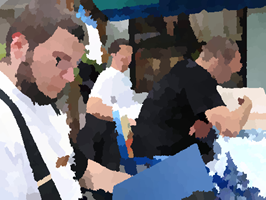
\includegraphics[width=\linewidth]{resources/segm_3_5.png}
			\caption{$\sigma = 3, \tau = 5$}
		\end{subfigure}
		\begin{subfigure}[b]{0.3\linewidth}
			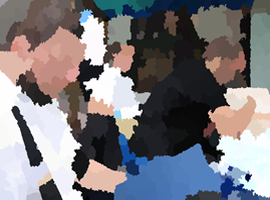
\includegraphics[width=\linewidth]{resources/segm_2_10.png}
			\caption{$\sigma = 2, \tau = 10$}
		\end{subfigure}
		\begin{subfigure}[b]{0.3\linewidth}
			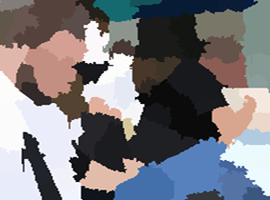
\includegraphics[width=\linewidth]{resources/segm_4_8.png}
			\caption{$\sigma = 4, \tau = 8$}
		\end{subfigure}
		\caption{Segmenting an image with different parameters}
		\label{fig:segmentation}
	\end{figure}
	
	The most suitable area for texture analysis was also determined experimentally. As can be observed in figure \ref{fig:texture} the 5x5 window offers a good detection of skin areas while the true positive rate goes down drastically for larger ones.
	
	\begin{figure}[h!]
		\centering
		\begin{subfigure}[b]{0.3\linewidth}
			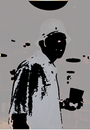
\includegraphics[width=\linewidth]{resources/texture_5_5.png}
			\caption{5x5}
		\end{subfigure}
		\begin{subfigure}[b]{0.3\linewidth}
			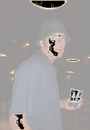
\includegraphics[width=\linewidth]{resources/texture_7_7.png}
			\caption{7x7}
		\end{subfigure}
		\begin{subfigure}[b]{0.3\linewidth}
			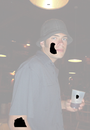
\includegraphics[width=\linewidth]{resources/texture_35_35.png}
			\caption{35x35}
		\end{subfigure}
		\caption{Texture detection with different windows}
		\label{fig:texture}
	\end{figure}
	
	I tried building color models in RGB, HSV and YCrCb and concluded that Bayesian color analysis obtains roughly the same results regardless of the color space chosen. For every pixel, I chose the maximum probability on a distance of 4 (similar to the bin size used in \cite{compaq}) on every feature. The threshold value can be used to control the TPR/FPR ratio.
	
	\subsection{Evaluation}
	The model was evaluated on the Compaq skin database in order to compare it with other approaches from literature. There is a difference however, in the number of images chosen for evaluation. While most references use a ~6000 image set for testing I used only 50 images due to time constraints.
	
	For each image in the testing set I calculated the True Positive Rate and the False Positive Rate by comparing each pixel from my output to the given mask and then I averaged the results.
	\begin{equation}
	\label{metrics}
	TPR = \frac{TP}{TP + FN}, \,\,\, FPR = \frac{FP}{FP + TN}
	\end{equation}
	Equation \ref{metrics} shows how those metrics were calculated. TP, FP, TN and FN stand for the numbers of true positives, false positives, true negatives and false negatives, respectively.
	
	\begin{table}[h!]
		\begin{center}
			\caption{Evaluation of the proposed model on the Compaq dataset}
			\label{tab:results}
			\begin{tabular}{c|c|c}
				\textbf{TPR} & \textbf{FPR} & \textbf{Threshold}\\
				\hline
				86.57\% & 28.48\% & 0.1\\
				76.29\% & 15.54\% & 0.25\\
				81.59\% & 21.29\% & 0.167\\
			\end{tabular}
		\end{center}
	\end{table}
	
	\section{Implementation}
	The application is made up out of five main modules, pictured in figure \ref{fig:main_modules}: segmentation, $color_analysis$, $texture_analysis$, evaluator and $application_gui$. The first three provide the basic image processing operations, the evaluator provides an interface for detection and performance measurements while the top module offers a visual interface for user convenience. I will present them in detail in separate sections.
	
	Some design decisions that influenced all modules are representing images as numpy arrays (a python library for array processing) and using named tuples as keys for all maps. 
	
	Named tuples are a feature implemented in the 'namedtuple' library and are an efficient way of representing keys. The two tuples used in this application are pixel position (x,y components) and color features.
	
	Most of the trivial image operations such as reading, writing and converting color space have been done using the 'opencv' library.
	
	All progress messages generated by the application are handled to a logger. This can be injected at startup to display images on console, file or pass them to another process to be displayed on a GUI.
	
	\begin{figure}[h!]
		\centering
		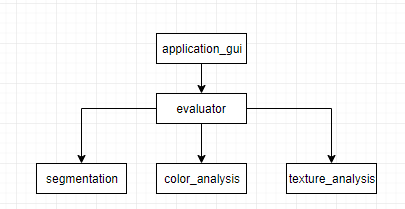
\includegraphics[]{design/main_modules.png}
		\caption{Main modules}
		\label{fig:main_modules}
	\end{figure}

	\subsection{The image segmentation module}
	An overview of this module can be seen in figure \ref{fig:image_segmentation}. The segmentation functionality is provided by the QuickshiftSegmentation class, which exposes two public methods, apply(image) and $get_superpixels(image)$, and takes the sigma and tau parameters in the constructor. The first method applies Quick shift segmentation on the image and returns an image where regions are visible, being colored with the same value as the root pixel. The second method returns a map containing all identified regions. The keys are roots pixels and the values their corresponding superpixels. 
	
	Regions are represented by the Superpixel class whose fields are: the initial image, position of the root pixel and a list of positions of all corresponding pixels.
	
	The Distances class encapsulates some methods used by the segmentation algorithm to calculate pixel and feature distances.
	
	\begin{figure}[h!]
		\centering
		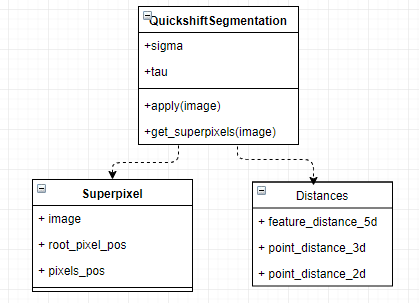
\includegraphics[]{design/image_segmentation.png}
		\caption{Image segmentation module}
		\label{fig:image_segmentation}
	\end{figure}

	\subsection{The color detection module}
	This module can be divided into two submodules: training, figure \ref{fig:color_train}, and detection, figure \ref{fig:color_detect}.
	
	In order to train a color detection model you must call the $train_spm_model$ static method which takes a SPMTrainConfiguration object. The configurable fields are the database (SFA or Compaq), the color space (RGB, HSV, YCrCb) and paths for resources. 
	
	Depending on the value of the database parameter the trainer creates either a SfaComponentExtractor or a CompaqComponentExtractor. Both of these classes provide a method $extract_components()$ that returns a BayesSPMComponents object, which encapsulates: the number of skin and non-skin pixels, a map with the number of apparitions for each pixel and a map with the number of apparitions as skin.
	
	The resulting model, a SPMModel object, is serialized into a file. It contains the selected color space and the components extracted on the previous step.
	
	\begin{figure}[h!]
		\centering
		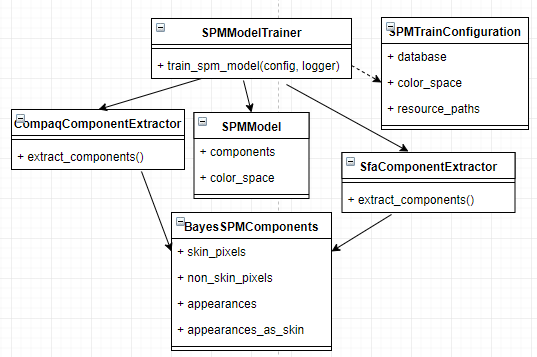
\includegraphics[]{design/color_train.png}
		\caption{Color detector training submodule}
		\label{fig:color_train}
	\end{figure}
	
	Depending on the input parameters the SPMDetectorFactory provides one of the following detectors: SimpleDetector, NeighborDetector or AverageOnSuperpixelDetector. The first one is the simplest approach as it calculates a probability for each pixel independently. The second, takes into account an area around each pixel. This simulates the histogram based approach with the difference that the considered pixel is always at the center of the area. The last detector calculates the average probability of a given superpixel.
	
	All detectors use the methods defined in ProbabilityCalculator through an intermediary layer. This proxy, CachedProbabilityCalculator, was created to speedup operations by caching probabilities. The need for memorizing these values arose from the fact that images usually contain a small subset of pixel values duplicated many times.
	
	\begin{figure}[h!]
		\centering
		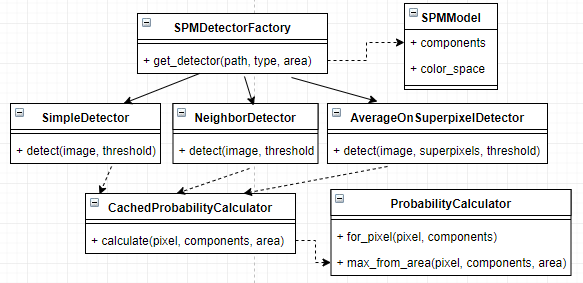
\includegraphics[]{design/color_detect.png}
		\caption{Color detection submodule}
		\label{fig:color_detect}
	\end{figure}
	
	\subsection{The texture analysis module}
	Similarly to the previous module, texture analysis can be divided into two submodules, one for training, figure \ref{fig:texture_train}, and one for detection, figure \ref{fig:texture_detect}.
	
	The model used in skin texture detection, TextureModel, has an attribute for extracting textural features from images (feature\_extractor), one for classifying those values (classifier), and label for interpreting the classifier's results (skin\_label). This model is trained by a HaralickModelTrainer which its parameters from a TextureTrainConfig object.
	
	In this project I only implemented a model based on Haralick's features but the design allows incorporating other methods. The HaralickModel extends the basic TextureModel and overrides the feature extraction method. It is trained by a HaralickModelTrainer which injects a HaralickFeatureExtractor, which encapsulates the feature extraction method taken from the mahotas library, and SvmClassifier, which trains a Support Vector Machine classifier using the sk\_learn library. The model trainer is also responsible for selecting a method of preparing the input data, in this case using the TrainDataPreparer class, which computes Haralick's features and appends the corresponding label.
	
	\begin{figure}[h!]
		\centering
		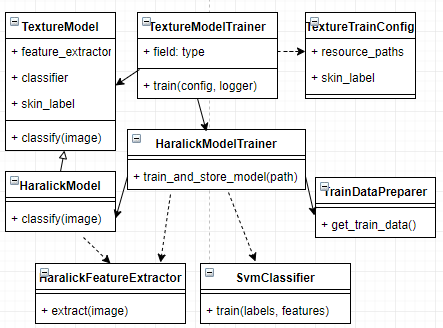
\includegraphics[]{design/texture_train.png}
		\caption{Texture detector trainer submodule}
		\label{fig:texture_train}
	\end{figure}

	There are two types of detectors available. The GridDetector slides a window over the image and classifies each of those blocks. The PerPixelDetector is a more precise approach because it builds a window around each pixel in the image and only marks the center pixel. Although the second approach gains a noticeable increase in precision, it is much slower than the first.

	\begin{figure}[h!]
		\centering
		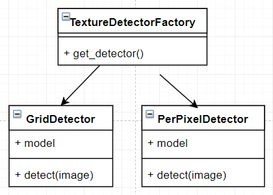
\includegraphics[]{design/texture_detect.png}
		\caption{Texture analysis submodule}
		\label{fig:texture_detect}
	\end{figure}
	
	\subsection{The evaluator module}
	
	The evaluator module has a simple structure, as seen in figure \ref{fig:evaluator}. The Evaluator class contains methods for evaluating a model(run\_simulation) and for applying it to an image(run\_detection). It takes as input a RunConfiguration object which contains informations about the desired skin and texture models and segmentation parameters.
	
	In order to evaluate the model some quality measures are applied for each analyzed picture. These methods include the false positive rate, true positive rate, precision, accuracy and recall and are implemented by the Stats class.
	
	\begin{figure}[h!]
		\centering
		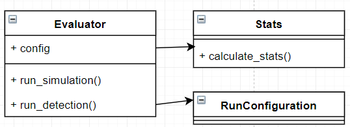
\includegraphics[]{design/evaluator.png}
		\caption{The evaluator module}
		\label{fig:evaluator}
	\end{figure}
	
	\subsection{User interface}
	
	The user interface was build using the tkinter library. This framework was designed to create modular applications. Consequently every window can be composed out of multiple frames, which are reusable components. The main views used in the application are visible in figure \ref{fig:gui}. The various configuration frames were left out of the diagram to avoid clutter.
	
	MainView is a tab-view component which is provides links to the application's main windows: color model training, texture model training, model evaluation, detection of a picture.
	
	Every component has a ProcessControlFrame which contains a FeedbackFrame and some buttons for starting and stopping operations. When the user presses the 'Start' button a new process is launched which performs the request and logs results into a queue. A monitoring thread reads that from the queue and passes it to the FeedbackFrame for displaying it on the screen. This approach allows the user to follow the application's progress while keeping the user interface decoupled from the algorithms.
	
	The detection view also contains an ImageDisplayFrame, which displays the input and the resulting image.
	
	\begin{figure}[h!]
		\centering
		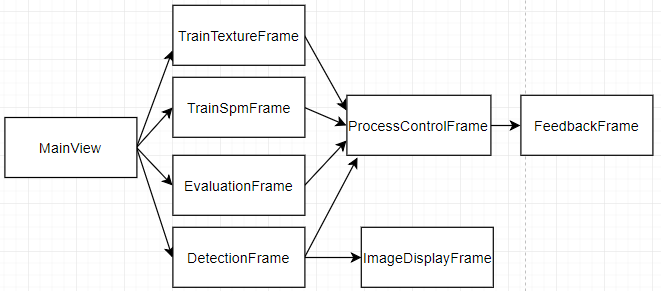
\includegraphics[]{design/gui.png}
		\caption{The user interface module}
		\label{fig:gui}
	\end{figure}
	
	\chapter{User manual}
	\section{Introduction}
	The goal of this application is to provide an easy-to-use and highly-configurable interface for training and evaluating skin detection models that share a core structure of image segmentation, color and texture analysis. The user can also test the created models on individual images. As the number of parameters for each task can be overwhelming the user can opt to use the default values that have already been set in each field.
	
	The application has 4 main windows accessible through a tab-view set in the top-left corner. The windows, detailed in the following sections, are the Evaluator, Train SPM, Train texture and Detection windows.
	
	\begin{figure}[h]
		\centering
		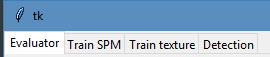
\includegraphics{manual/tab_view.png}
		\caption{The tab-view main menu}
	\end{figure}

	\section{Detection view}
	This view allows the user to test the model on individual images and get visual feedback. The resulting image will be displayed on the screen with a black mask that marks the identified pixels. This window provides a quick way to evaluate a model or to make a demonstration.
	
	If you want to apply the model to a single image you must specify the detection parameters, or go with the default ones, provide a path to the input image (bottom frame on the left side of the screen) and click ‘Start experiment’. The initial image and the result will be displayed on the frames on the right side of the screen. The other configuration frames are explained in detail in section \todo{link to section}. 
	
	On the middle of the screen, below the buttons for controlling the experiment, you will see updates of the detection process. A progress bar will follow the time consuming operations: segmentation, color and texture analysis.

	\begin{figure}[h!]
		\centering
		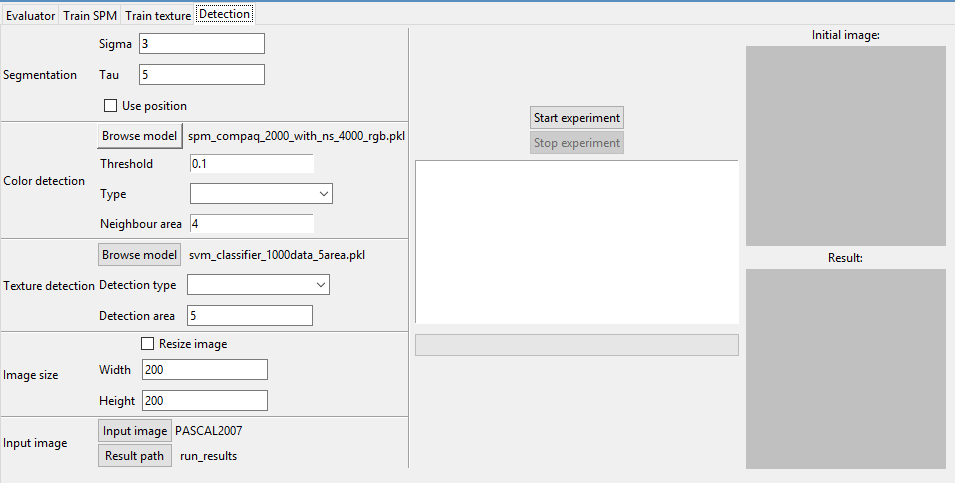
\includegraphics[width=\linewidth]{manual/detection_view.png}
		\caption{Detection view}
	\end{figure}

	\section{Evaluator view}
	
	This screen allows the user to evaluate the performance of the final model and follow the progress in real time. The selected model can be configured in various ways which will be presented in detail in the common configurations section \todo{link to section}.
	
	\begin{figure}[h!]
		\centering
		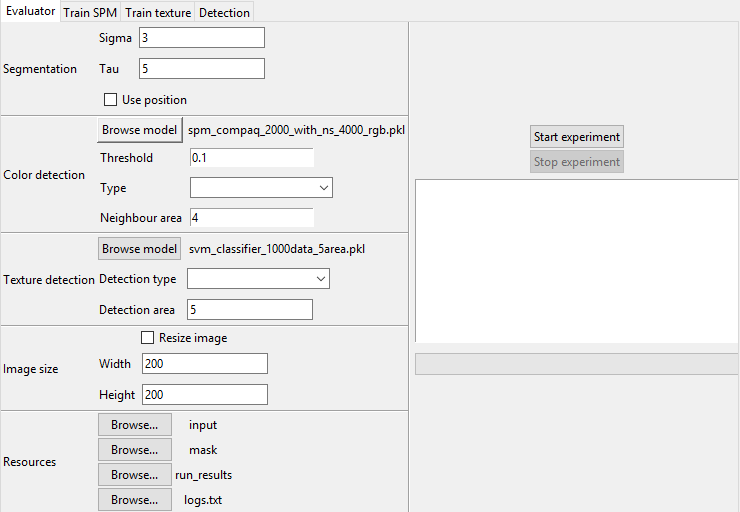
\includegraphics[width=\linewidth]{manual/evaluator_view.png}
		\caption{Evaluator view}
	\end{figure}

	The application applies the selected model to images from the provided folders. Input images can have any size and name. Masks should have the same size and name as their corresponding input and should mark skin pixels in black (0, 0, 0). The paths where execution logs and run results are stored are also customizable.
	
	To begin evaluation you must press ‘Start experiment’. The frame below the button displays information about the currently processed picture, the operation in progress and evaluation results. 
	
	A progress bar will indicate the status of each action applied to the image. The main actions are, in order: image segmentation (consisting of density computation, neighbor linking and superpixel extraction), color detection (Bayes SPM), texture analysis (Haralick feature, combination of results and metrics calculation. Images obtained for each step (color, texture and their combination) are all saved in the results folder, to facilitate the identification of cases for which the model does not perform as expected.
	
	After each picture is analyzed by the model, the performance metrics(true positive rate, false positive rate, true negative rate, false negative rate, accuracy, precision and recall) are displayed on the screen and saved to a file.
	The application builds a csv file containing metrics from each processed picture, that can be used to obtain overall results.
	
	\section{}
	
	\chapter{Conclusions}
	
	\newpage
	\bibliography{references}
	\bibliographystyle{ieeetr}
\end{document}